% GNUPLOT: LaTeX picture with Postscript
\begingroup
  \makeatletter
  \providecommand\color[2][]{%
    \GenericError{(gnuplot) \space\space\space\@spaces}{%
      Package color not loaded in conjunction with
      terminal option `colourtext'%
    }{See the gnuplot documentation for explanation.%
    }{Either use 'blacktext' in gnuplot or load the package
      color.sty in LaTeX.}%
    \renewcommand\color[2][]{}%
  }%
  \providecommand\includegraphics[2][]{%
    \GenericError{(gnuplot) \space\space\space\@spaces}{%
      Package graphicx or graphics not loaded%
    }{See the gnuplot documentation for explanation.%
    }{The gnuplot epslatex terminal needs graphicx.sty or graphics.sty.}%
    \renewcommand\includegraphics[2][]{}%
  }%
  \providecommand\rotatebox[2]{#2}%
  \@ifundefined{ifGPcolor}{%
    \newif\ifGPcolor
    \GPcolorfalse
  }{}%
  \@ifundefined{ifGPblacktext}{%
    \newif\ifGPblacktext
    \GPblacktexttrue
  }{}%
  % define a \g@addto@macro without @ in the name:
  \let\gplgaddtomacro\g@addto@macro
  % define empty templates for all commands taking text:
  \gdef\gplbacktext{}%
  \gdef\gplfronttext{}%
  \makeatother
  \ifGPblacktext
    % no textcolor at all
    \def\colorrgb#1{}%
    \def\colorgray#1{}%
  \else
    % gray or color?
    \ifGPcolor
      \def\colorrgb#1{\color[rgb]{#1}}%
      \def\colorgray#1{\color[gray]{#1}}%
      \expandafter\def\csname LTw\endcsname{\color{white}}%
      \expandafter\def\csname LTb\endcsname{\color{black}}%
      \expandafter\def\csname LTa\endcsname{\color{black}}%
      \expandafter\def\csname LT0\endcsname{\color[rgb]{1,0,0}}%
      \expandafter\def\csname LT1\endcsname{\color[rgb]{0,1,0}}%
      \expandafter\def\csname LT2\endcsname{\color[rgb]{0,0,1}}%
      \expandafter\def\csname LT3\endcsname{\color[rgb]{1,0,1}}%
      \expandafter\def\csname LT4\endcsname{\color[rgb]{0,1,1}}%
      \expandafter\def\csname LT5\endcsname{\color[rgb]{1,1,0}}%
      \expandafter\def\csname LT6\endcsname{\color[rgb]{0,0,0}}%
      \expandafter\def\csname LT7\endcsname{\color[rgb]{1,0.3,0}}%
      \expandafter\def\csname LT8\endcsname{\color[rgb]{0.5,0.5,0.5}}%
    \else
      % gray
      \def\colorrgb#1{\color{black}}%
      \def\colorgray#1{\color[gray]{#1}}%
      \expandafter\def\csname LTw\endcsname{\color{white}}%
      \expandafter\def\csname LTb\endcsname{\color{black}}%
      \expandafter\def\csname LTa\endcsname{\color{black}}%
      \expandafter\def\csname LT0\endcsname{\color{black}}%
      \expandafter\def\csname LT1\endcsname{\color{black}}%
      \expandafter\def\csname LT2\endcsname{\color{black}}%
      \expandafter\def\csname LT3\endcsname{\color{black}}%
      \expandafter\def\csname LT4\endcsname{\color{black}}%
      \expandafter\def\csname LT5\endcsname{\color{black}}%
      \expandafter\def\csname LT6\endcsname{\color{black}}%
      \expandafter\def\csname LT7\endcsname{\color{black}}%
      \expandafter\def\csname LT8\endcsname{\color{black}}%
    \fi
  \fi
  \setlength{\unitlength}{0.0500bp}%
  \begin{picture}(5040.00,3600.00)%
    \gplgaddtomacro\gplbacktext{%
      \csname LTb\endcsname%
      \put(472,360){\makebox(0,0)[r]{\strut{}}}%
      \put(472,623){\makebox(0,0)[r]{\strut{}400}}%
      \put(472,827){\makebox(0,0)[r]{\strut{}}}%
      \put(472,994){\makebox(0,0)[r]{\strut{}}}%
      \put(472,1134){\makebox(0,0)[r]{\strut{}}}%
      \put(472,1256){\makebox(0,0)[r]{\strut{}800}}%
      \put(472,1364){\makebox(0,0)[r]{\strut{}}}%
      \put(472,1460){\makebox(0,0)[r]{\strut{}1000}}%
      \put(472,2094){\makebox(0,0)[r]{\strut{}2000}}%
      \put(472,2465){\makebox(0,0)[r]{\strut{}}}%
      \put(472,2728){\makebox(0,0)[r]{\strut{}4000}}%
      \put(472,2931){\makebox(0,0)[r]{\strut{}}}%
      \put(472,3098){\makebox(0,0)[r]{\strut{}}}%
      \put(472,3239){\makebox(0,0)[r]{\strut{}}}%
      \put(788,140){\makebox(0,0){\strut{}}}%
      \put(2002,140){\makebox(0,0){\strut{}}}%
      \put(2712,140){\makebox(0,0){\strut{}}}%
      \put(3215,140){\makebox(0,0){\strut{}}}%
      \put(3606,140){\makebox(0,0){\strut{}}}%
      \put(3925,140){\makebox(0,0){\strut{}}}%
      \put(4195,140){\makebox(0,0){\strut{}}}%
      \put(4429,140){\makebox(0,0){\strut{}}}%
      \put(-100,1799){\rotatebox{-270}{\makebox(0,0){\strut{}runtime (ms)}}}%
      \put(2569,3569){\makebox(0,0){\strut{}Laplace on 2xQuad Core 2.0GHz Intel Harpertown}}%
      \put(788,2835){\rotatebox{-27}{\makebox(0,0)[l]{\strut{}Safe Get}}}%
      \put(788,2552){\rotatebox{-26.5}{\makebox(0,0)[l]{\strut{}Unsafe Get}}}%
      \put(788,1935){\rotatebox{-16.5}{\makebox(0,0)[l]{\strut{}Unsafe Unrolled Get}}}%
      \put(788,1312){\rotatebox{-6}{\makebox(0,0)[l]{\strut{}Safe Unrolled Stencil}}}%
      \put(788,689){\makebox(0,0)[l]{\strut{}Handwritten C with GCC 4.4.3}}%
    }%
    \gplgaddtomacro\gplfronttext{%
    }%
    \gplbacktext
    \put(0,0){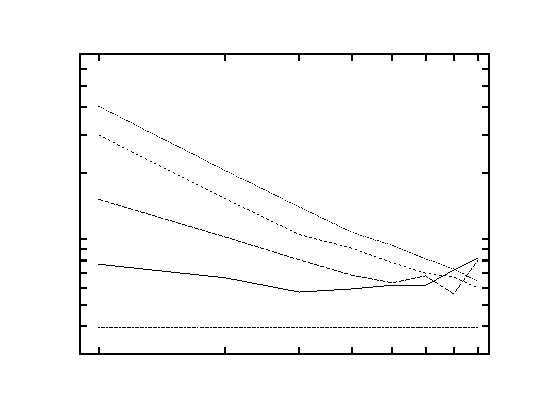
\includegraphics{data/laplace/tesla}}%
    \gplfronttext
  \end{picture}%
\endgroup
